\documentclass[conference]{IEEEtran}
\IEEEoverridecommandlockouts
% The preceding line is only needed to identify funding in the first footnote. If that is unneeded, please comment it out.
\usepackage{cite}
\usepackage{breqn}
\usepackage{amsmath,amssymb,amsfonts}
\usepackage{algorithmic}
\usepackage{graphicx}
\usepackage{xfrac}
\usepackage{textcomp}
\usepackage{xcolor}
\def\BibTeX{{\rm B\kern-.05em{\sc i\kern-.025em b}\kern-.08em
    T\kern-.1667em\lower.7ex\hbox{E}\kern-.125emX}}
\begin{document}

\title{Natural Disaster Geospatial Damage Assessment\\
}

\author{\IEEEauthorblockN{\textbf{Billy Ermlick \qquad Nick Newman \qquad Devayani Pawar \qquad Tyler Richardett}}
\IEEEauthorblockN{{Department of Statistics} \\
{George Mason University} \\ 
{Fairfax, VA 22030} \\
\texttt{\{wermlick, nnewman7, dpawar, tricha3\}@gmu.edu}}

}

\maketitle

\begin{abstract}
When a natural disaster occurs, damaged regions rely on timely damage assessments to receive relief. Currently, this is a slow and laborious process, during which groups such as the Federal Emergency Management Agency (FEMA) conduct on-the-ground evaluations to form fiscal estimates. This project attempts to expedite relief efforts by applying computer vision algorithms to satellite images to quickly and accurately estimate physical and fiscal damage caused by natural disasters. The data used for this analysis consists of satellite images from six types of natural disasters gathered from the xBD dataset provided by the Defense Innovation Unit. Modeling efforts include the use of connected U-Nets and Mask RCNN for building localization and damage classification, with a pixel-based financial model capable of outputting financial costs according to the United States National Grid (USNG) coordinate system. A proof-of-concept web application is presented to summarize the results of the analysis. This application provides an efficient method for fiscal evaluation and can enable aid to be rapidly provided to areas in need.
\end{abstract}

\begin{IEEEkeywords}
Natural Disaster, U-Net, Computer Vision, United States National Grid, Financial Modeling, Mask R-CNN, Remote Sensing, Convolutional Neural Networks
\end{IEEEkeywords}

\section{Introduction}
Natural disasters are costly and time-sensitive events that have the potential to wreak havoc on an entire region. Currently, the Federal Emergency Management Agency (FEMA) and other agencies conduct damage assessments to determine the extent of damage in a region following a natural disaster, but these are often slow, unsafe, and laborious processes. The regions are dependent upon the assessments, and the funding that follows, in order to rebuild their lost infrastructure. These funds can take many months, or in some cases years, to reach the effected community. This inefficient process provides further undue hardship upon the residents of the region. 

 As disasters typically interrupt communication and travel paths for damage surveyors conducting on-the-ground assessments, use of remote sensing means can be used to improve the speed and safety of assessments. High resolution satellite imagery is available immediately following a natural disaster and shows the details of specific damage conditions from the event. FEMA and other agencies presently manual search and annotate these images for damage or obstructions, and make limited use of automatic forms of analysis.  Due to the scale of most disasters, manually searching and annotating these images for damage or obstructions is a tenuous process for analysts and can benefit from improved automation. In addition, FEMA in particular utilizes the United States National Grid coordinate system to summarize their assessment results for disaster response. Integration of the output from automated assessment techniques into this coordinate system would speed up the analysis process and aid in providing fast, accurate, safely obtained, damage summaries.  
 


We propose a way this remote sensing analysis process can be efficiently improved by leveraging computer vision methods. We use the xBD dataset, provided by The Defense Innovation Unit, to train our classifier on this problem. This dataset, released in July of 2019, is the largest building damage dataset to date, containing over 20,000 images with over 800,000 building annotations \cite{a1}. Deep Convolutional Neural Network architectures are used to simultaneously localize the buildings in these images and classify the damage inflicted upon them. After building locations and damage classifications are obtained, fiscal costs of the damage are estimated using a pixel-based financial model and summarized according to the United States National Grid coordinate system.

This paper introduces a novel web application that uses satellite imagery to effectively estimate and summarize the fiscal damage to a region impacted by a natural disaster as shown in Fig.~\ref{appbig}. This tool, if implemented, can efficiently reduce the fiscal evaluation and relief process required by FEMA, and in turn, enable these affected regions to quickly receive the funds they desperately require.

 \begin{figure}[htbp]
\centering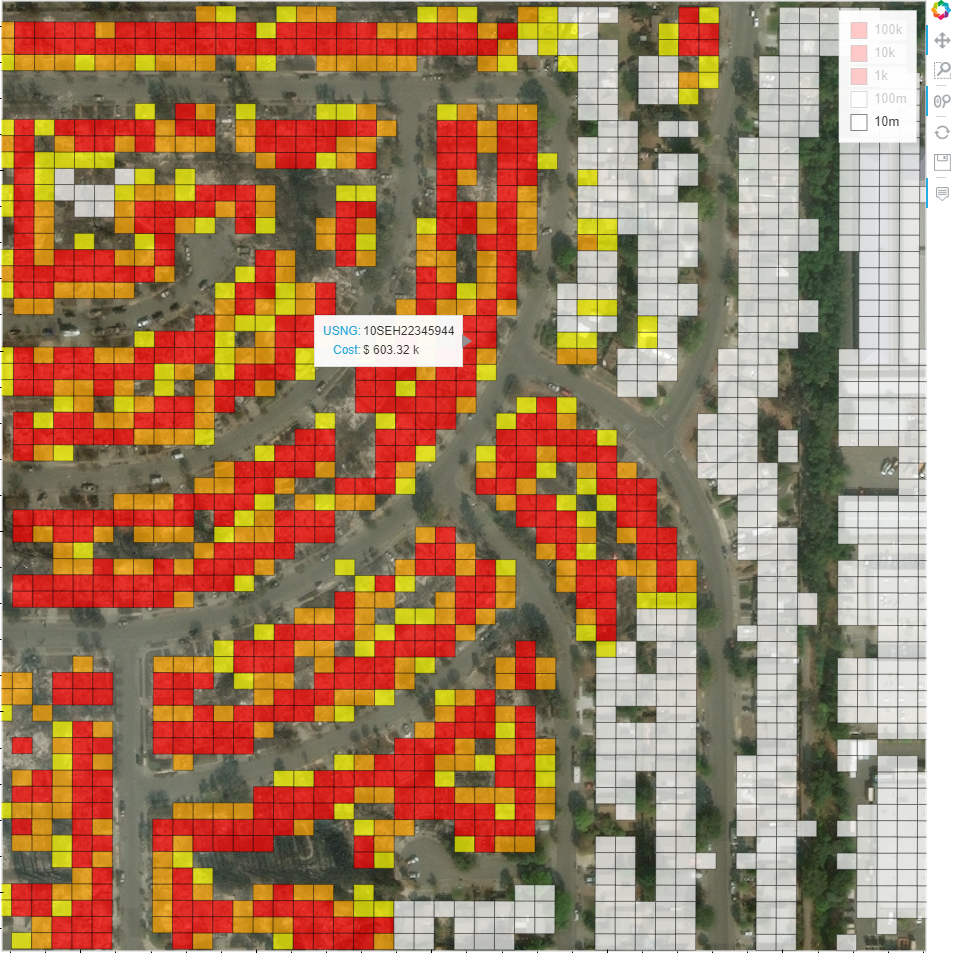
\includegraphics[width=1\linewidth]{AppImage.png}
\caption{Pixel-based Financial Damage Assessment Application}
\label{appbig}
\end{figure}


\section{Related Work}

Several studies have used chipped, pre- and post-disaster satellite images to remotely assess the degree of damage sustained by physical structures during and after such events \cite{a3, a4, a5}. Fujita et al. \cite{a3} trained CNNs from scratch to localize buildings and classify whether they had survived or were washed away by the 2011 Tōhoku tsunami. Xu et al. \cite{a4} compared the performance of four AlexNet architectures\cite{a6} in detecting whether buildings suffered any level of damage, following one of three major earthquakes. This study originally sought to classify post-disaster buildings based on the severity of damage observed, but the authors abandoned this approach due to noisy assessments in their dataset. Doshi et al. \cite{a5} applied a framework for change detection over larger, gridded regions, using CNNs, to quantify the impact of one flooding and one fire event. Their work covered roads and buildings but left the extension of other natural or man-made structures for future exploration.

Conversely, other studies explore the merits of only using post-disaster satellite images for remote damage detection \cite{a7}. As Fujita et al. \cite{a3} discovered in their work, high-quality, pre-disaster satellite images will not always be available for every region impacted by a significant natural disaster. Ji et al. \cite{a7} used a SqueezeNet architecture\cite{a8} on post-disaster satellite images to detect whether physical structures had collapsed following the 2010 Haiti earthquake.

In contrast to this related work, our study takes the model outputs one step further---applying spatiotemporal property value estimates to produce region-by-region, dollar-value damage estimations according to the USNG.  

\section{Predictive Modeling Process}
\subsection{Dataset}
The xBD dataset contains images across 19 natural disasters consisting of events such as volcanic eruptions, fires, floods, hurricanes, etc. Each image has a resolution of 1024 by 1024 pixels. The dataset also introduces a Joint Damage Scale, which is an attempt to create consistency by having a unified damage scale across natural disasters \cite{a1}. Each pixel in the images is labeled on a scale of 0-3, corresponding to the amount of damage. In an effort to create a unified model that simultaneously performs localization and classification, we have slightly adjusted these metrics to the following: 0 = No Building, 1 = No Damage, 2 = Minor Damage, 3 = Major Damage, 4 = Destroyed.

The dataset is conveniently provided with pre-split train, holdout, and test image sets. We combined the holdout and test sets to use as one unified test set, which allowed us to be more confident in the results of our predictions. Rather than having a specifically held-out validation set, we opted to use a random subset of the training set for validation after every epoch. While the results were not as consistent as having a singular validation set, it helped to alleviate any sort of bias in the results due to the heavy class imbalance present in the training set. 

Minimal preprocessing was needed for the dataset. Each pre- and post-disaster image pair is associated with a JSON file containing a list of polygons representing the locations of the buildings within the images. Each of these polygons is also linked to a label containing the post-disaster damage level. We used these polygon coordinates to create image masks for each set of images. The resulting masks were of shape (1024, 1024, 5), with the final dimension consisting of binary numbers, representing of the presence of a particular class in the relative pixel.

\subsection{U-Net Architecture}
Because the goal of this endeavor was to develop a proof-of-concept application, rather than a one-off prediction, we focused on maximizing the speed of the model during inference time. Creating separate models for building localization and classification would have significantly increased the time from input to output, something that is unacceptable when delivering an application to an end user. This led us to create a single model to simultaneously perform localization and classification.

Due to its success in the domain of image segmentation, we decided to use a U-Net architecture for this project \cite{a2}. Normally, the standard U-Net architecture takes an image as input and returns that same image segmented into regions based on the classes specified during the network initialization. With this structure, only one image can be processed at a time, which would have required the use of two U-Nets - one to generate masks for the buildings and another to generate damage predictions. To remedy this issue, we created a U-Net architecture with an additional encoder branch, allowing for dual image input. This not only streamlines the inference process, but enhances the training process as well. Through this method, the network is able to learn the difference between the pre- and post-disaster images, and therefore more effectively classify the level of damage.

The input for the network consists of pre- and post-disaster image tensors of shape (1024, 1024, 3). During the encoder stage, the images were simultaneously processed by the network, each image convolving through separate layers, but sharing the same kernel weights. At each step of the decoder stage, the layers are concatenated with the difference between the outputs of the pre- and post-disaster image encoder layers. The output of the model is a tensor of shape (1024, 1024, 5), with each channel in the final dimension representing one of the distinct classes. The indices of the maximum values across this axis are returned to receive the predicted class for each pixel of the image. This results in a tensor of shape (1024, 1024) where each pixel is a distinct class. A visual representation of the network is shown in Figure~\ref{fig:unet}. The entire network was implemented from scratch using TensorFlow and Keras.


\begin{figure}[h!]
\centering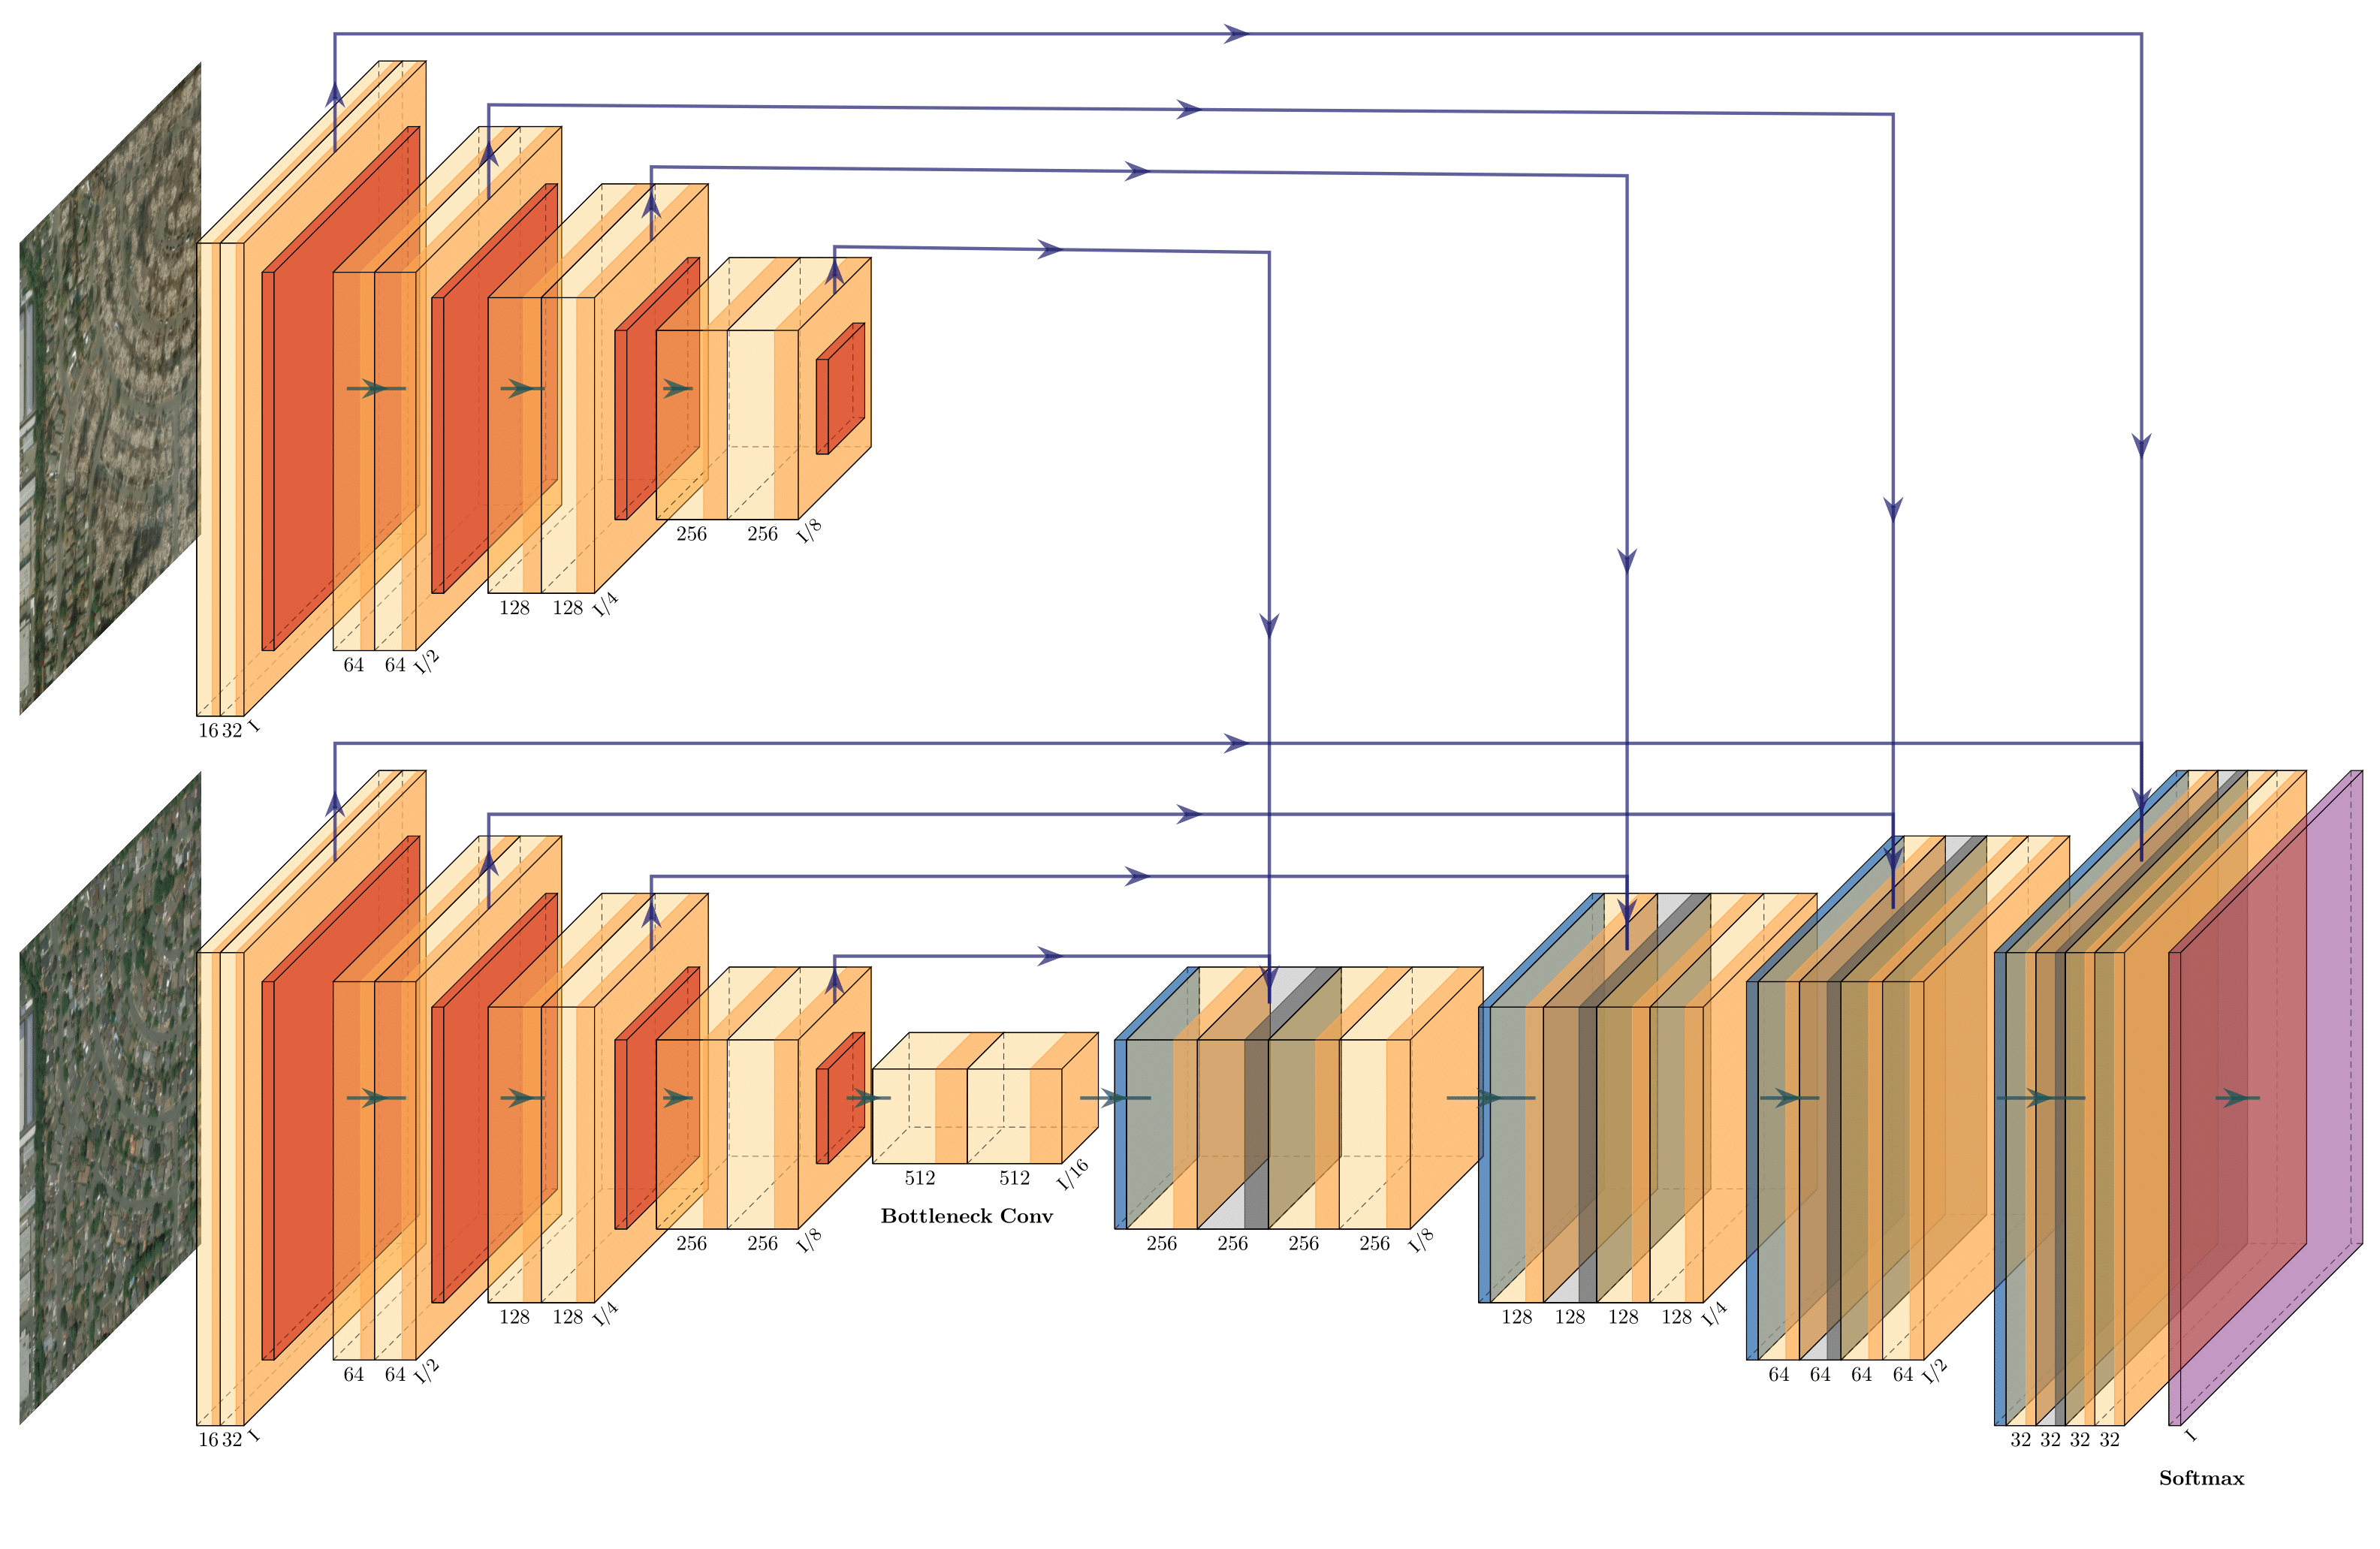
\includegraphics[width=1\linewidth]{unet.pdf}
\caption{U-Net architecture used}
\label{fig:unet}
\end{figure}

\subsection{Mask R-CNN Architecture}
Mask R-CNN\cite{a18} solves multi-bounding box problems and semantic segmentation independently, which efficiently solves the task of instance segmentation. It is a simple model that combines two extremely powerful existing models together - Faster R-CNN and semantic segmentation. In this model, first, we pre-train a Deep-CNN on image classification tasks which proposes regions. From there, Region Proposal Network is able to look at the feature map and get a set of bounding boxes that would essentially have an object of relevance by using selective search. 

The most important component of this model, which helps Mask R-CNN to implement pixel-level segmentation, is its RoI Align layer. This layer uses bilinear interpolation to avoid the misalignments caused by RoI Pool. The semantic segmentation model is implemented on each bounding box detected, which essentially is a binary classifier classifying object as 1 and background as 0. The model branches into 3 output layers: a softmax estimator of K + 1 classes outputting a discrete probability distribution per RoI, a bounding-box regression model which predicts offsets relative to the original RoI for each of K classes, and a separate branch that generates Mask for each RoI and class. The multi-task loss function of Mask R-CNN combines the loss of classification, localization, and segmentation mask. Here, classification loss is a log loss function over two classes while localization loss is a  smooth L1 loss and  Mask loss is a binary cross-entropy loss.

For our particular dataset, we combine pre- and post-disaster images to get 6-channel input image for damage detection. Experimentation with semantic segmentation in place of instance segmentation was also conducted and found to not be effective in detecting small buildings. We use pre-trained weights initially trained on the same model for detecting buildings. For Damage detection, we consider four classes: No Damage, Minor Damage, Major Damage, and Destroyed plus one class for a background. Here, super-category would be building (1)/BackGround(0).


\begin{figure}[h!]
\centering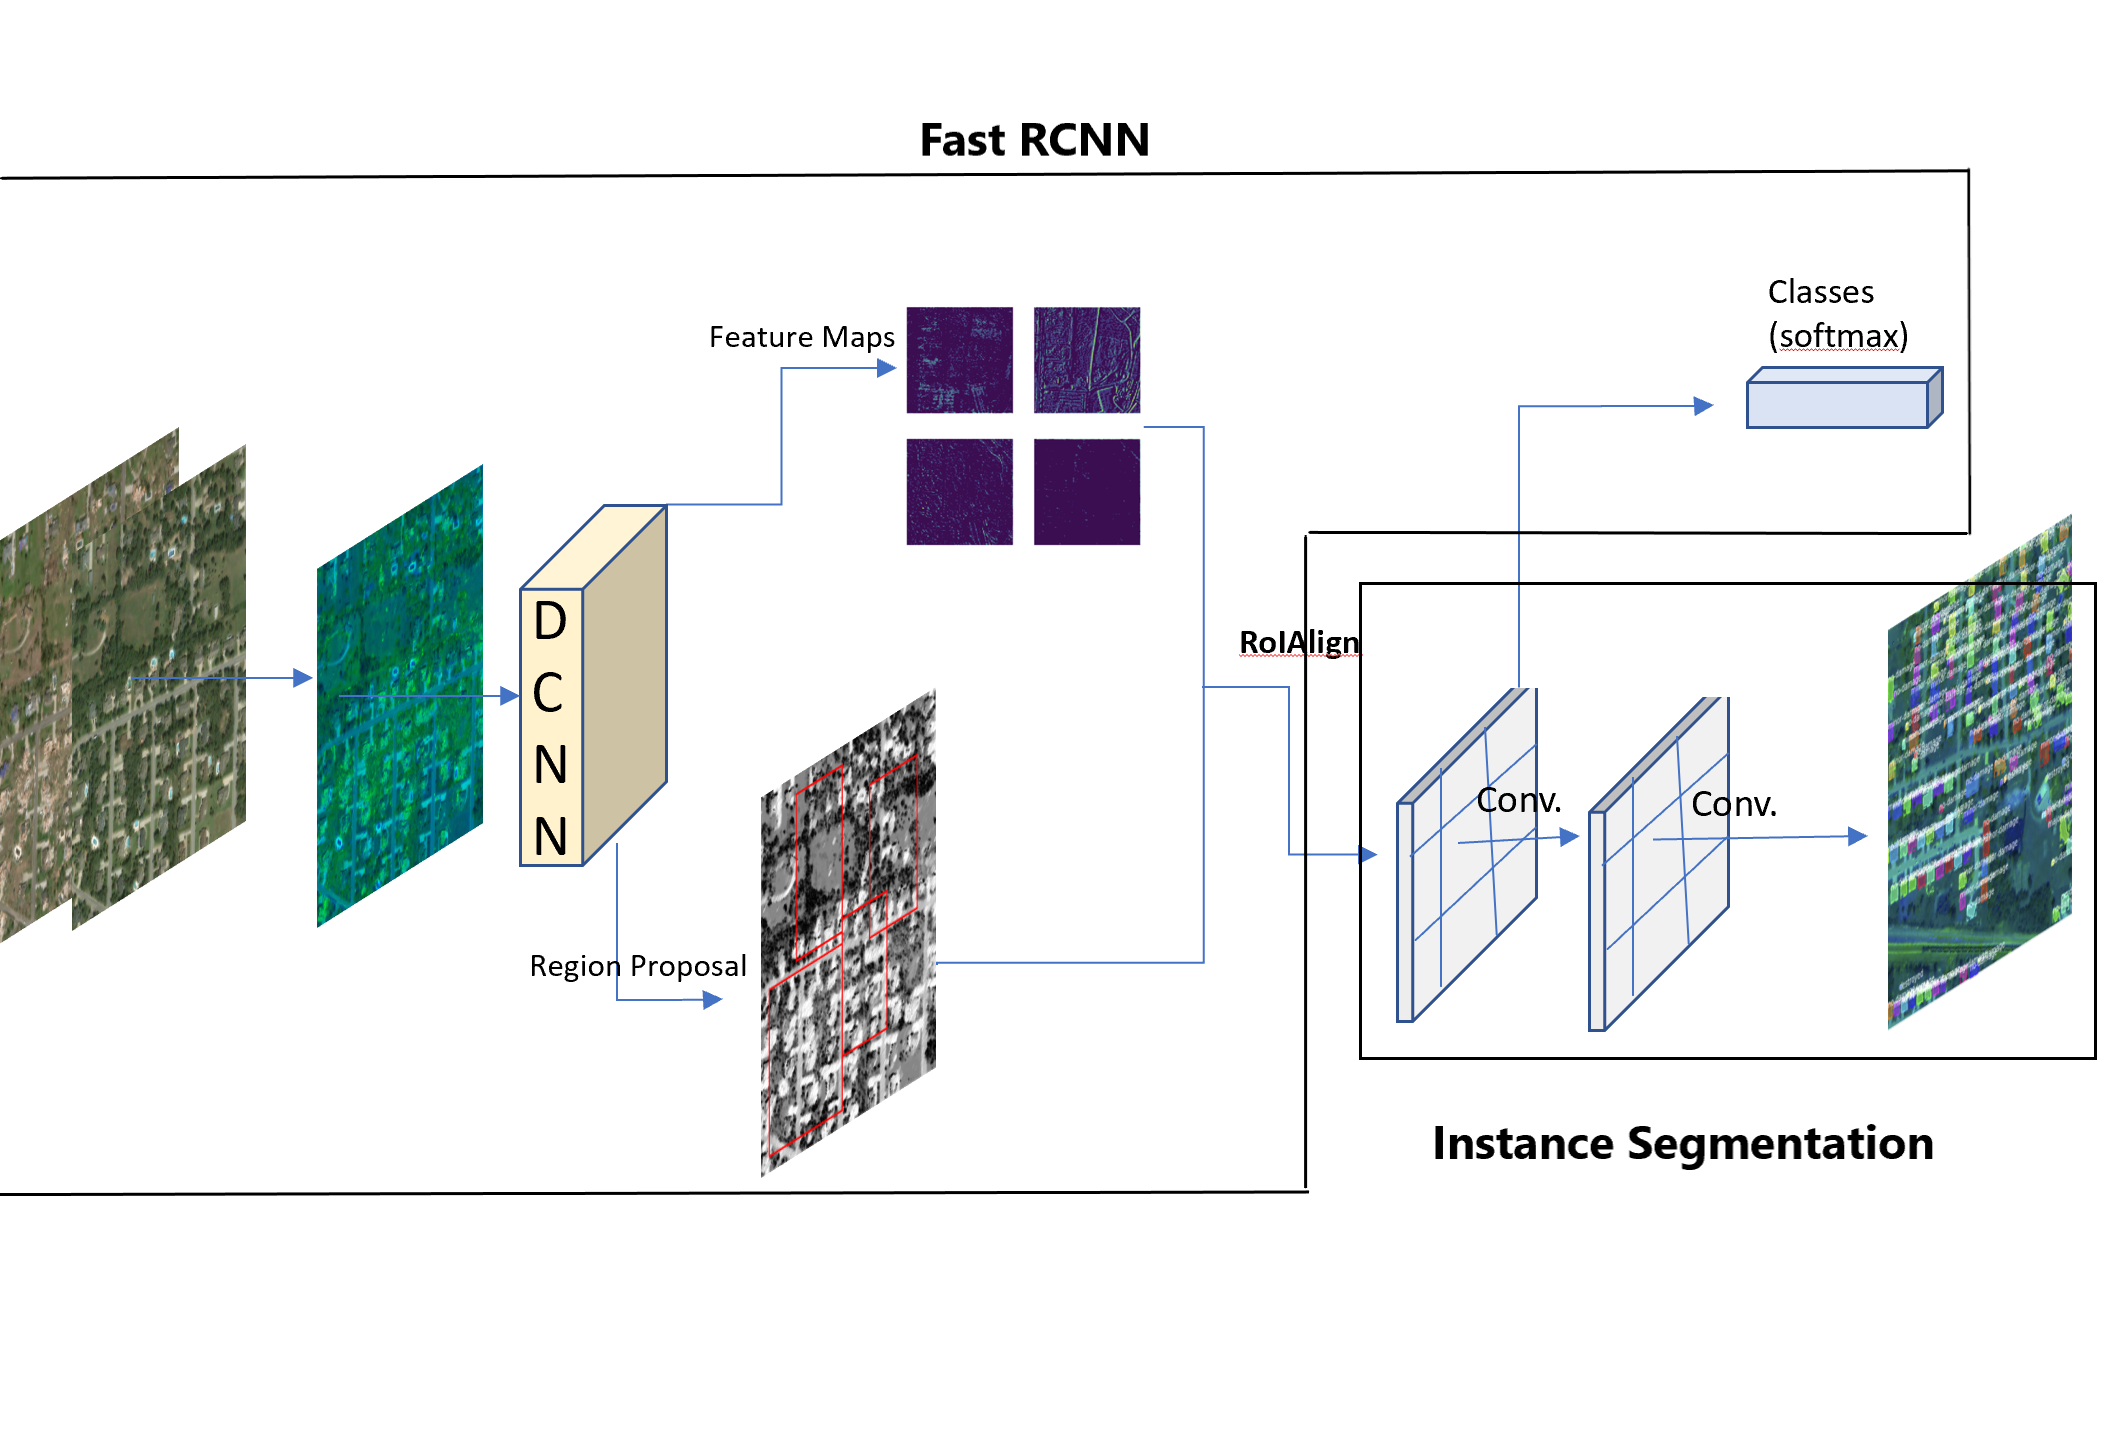
\includegraphics[width=1\linewidth]{MaskRCNN.png}
\caption{Mask-RCNN architecture}
\label{fig:MaskRCNN}
\end{figure}

\subsection{Methods}
As shown in Table~\ref{pixels}, the training set images contain a significant amount of class imbalance. We took a few different measures to counteract the class imbalance present in the dataset. The loss functions consisted of a combination of generalized Dice loss\cite{a9} and cross entropy with class weights. Using weights with cross entropy allowed us to place more of a penalty on the misclassification of certain classes. Originally, predictive performance on minor and major damage was poor; therefore, any image containing pixels in either of these classes was oversampled to assist in learning. We also tracked precision and recall during training to monitor, in real time, the effects of different hyperparameters on performance.

\begin{table}[htbp]
\begin{center}
\begin{tabular}{||c|c|c||}
\hline
\textbf{Class} & \textbf{Damage Level} & \textbf{Percentage of Pixels} \\
\hline\hline
0 & No Building & 97.632\% \\ 
1 & No Damage & 1.807\% \\
2 & Minor Damage & 0.204\% \\
3 & Major Damage & 0.219\% \\
4 & Destroyed & 0.138\% \\
\hline
\end{tabular}
\end{center}
\caption{Damage level frequencies by percentage of pixels}
\label{pixels}
\end{table}



\section{Financial Modeling Process}

\subsection{United States National Grid Mapping}
The United States National Grid (USNG) is a hierarchical grid system adopted in 2009 as the standard for disaster response operational maps provided by FEMA \cite{a10}. These grids are defined at various levels of precision, the smallest grids being one square meter in area and the largest covering six degrees latitude by eight degrees longitude. The grid lines follow latitude and longitude lines and essentially provide a 15 character reference system over-top of the Universal Transverse Mercator (UTM) coordinate system. The USNG is for all intents and purposes a subset of the Military Grid Reference System (MGRS), the USNG being defined over the United States and the MGRS the entire world. An image of the United States National Grid is found in Fig.~\ref{usngmap} \cite{a10}.

\begin{figure}[h]
\centering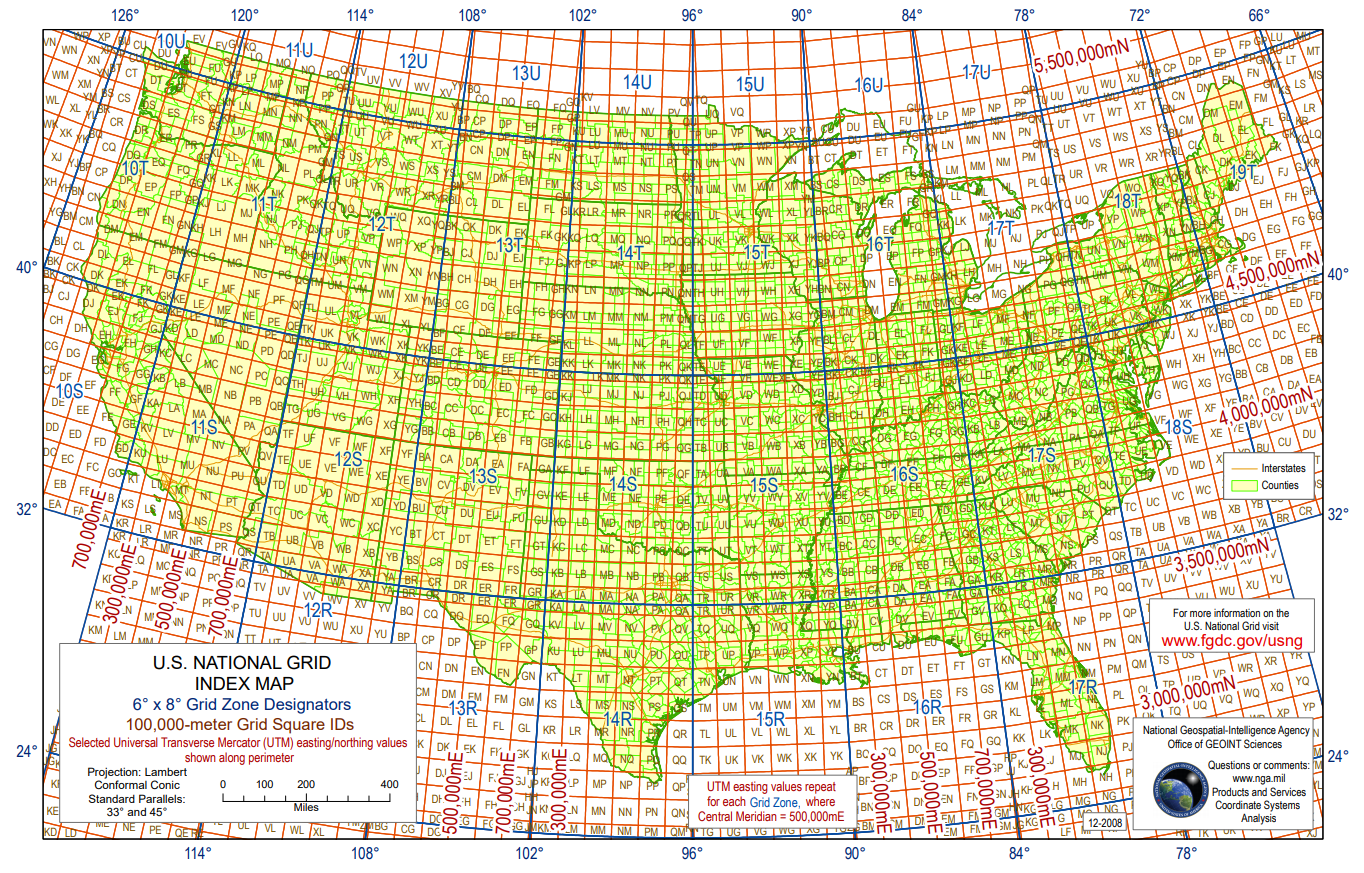
\includegraphics[width=1\linewidth]{USNG.png}
\caption{United States National Grid}
\label{usngmap}
\end{figure}

While shape-files of the USNG exist \cite{a11}, importable python libraries which allow for fast plotting of grid polygon coordinates are not readily available. The \emph{mgrs} library is the nearest python package \cite{a12} that is made use of in this effort. This library allows fast conversion of lat/lon coordinates into the MGRS coordinate grid reference system down to one meter precision and conversely returns the lat/lon of the southwest corner of a particular MGRS grid. Polygon coordinates of each grid coordinate is not provided within the function, as the C library on which it is built, GeoTrans, does not provide this functionality \cite{a13}. Utilizing the \emph{mgrs} library and knowledge of the MGRS/USNG coordinate system, a function can be developed to determine polygon coordinates of USNG grids to a high degree of precision. 

In greater detail, a grid of the USNG is characterized by a 15 character string as shown in Fig.~\ref{usngidentifier}. The Grid Zone Designation (GZD) defines a 6' longitude by 8' latitude area and designates the largest units within the system as mentioned earlier. The main group identifier is a one hundred kilometer area with two letters, the first which varies from A-Z west-east and the second which varies from A-V south-north (the letters I and O are excluded to avoid confusion with "1" and "0"). The set of numbers which follow detail further zones within the GZD and main group, specifying an easting and northing value with reference to the south west corner of the main group grid. Additional digits in the easting and northing value pairs specify the level of precision within the main group grid, with ("\#\#\#\#\#" "\#\#\#\#\#") indicating a precision of one meter, ("\#" "\#") a precision of ten kilometer and values in-between representing respective levels. 

\begin{figure}[ht]
\centering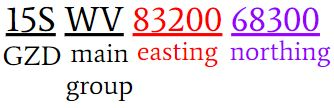
\includegraphics[width=0.4\linewidth]{USNGidentifier.JPG}
\caption{United States National Grid coordinate identifier}
\label{usngidentifier}
\end{figure}

The approach for obtaining grid polygon coordinates is straightforward in theory. The \emph{mgrs} package provides the southwestern coordinate of a particular grid directly, obtaining the coordinates of the other three coordinates will yield the full polygon. Using the regular repetition of main group and easting/northing values, the polygon for a particular grid can be obtained by first finding the grids directly north, northeast, and east of the grid of interest. Once these adjacent grids are known, the \emph{mgrs} can then be used to determine the lat/lons of the southwest corner of each of these grids, thereby obtaining the lat/lon positions of the four corners of the particular grid of interest.

Finding adjacent grids for grids specified at the main group level of precision can be done by traveling to the next letter for the first and second letter in the main group to move to grids east or north of the present grid, respectively. Progressing both letters provides the nearest northwestern grid. Adjacent grids at precision less than ten kilometers are simpler, as adding one to the easting or northing value will obtain the eastern/northern grid in a similar fashion. In this way, a plotting function is built which can quickly provide a polygon of a particular USNG grid. 

Edge cases exist for the present approach, some of which prove difficult to resolve perfectly. Easily managed cases consist of changes at precision below ten kilometers at the edge of main group grid boundaries. These take the form of an easting or northing value ending in nine (e.g., "9", or "9999"). These cases are resolved by moving to the appropriate adjacent main group and zeroing out the affected easting or northing value. More difficult edge cases exist within the changing of GZD zones, as these changes alter the main group letter progression pattern. These issues were resolved by using an approximation for longitudinal cross-over values as these GZD zone changes occur along regular longitudinal lines. While not perfectly accurate for all levels of precision, this assumption is sufficient for fast visualization purposes.

\subsection{Financial Model}
To estimate the expected cost associated with predicted damage levels, a simple financial model was developing using a pixel area based approach based on building square footage. The xBD data provided lat/lon polygons of each building within the competition, enabling their areas to be determined. Zillow data provided price per square footage costs for each zip-code using the 2018 Zillow Home Value Index (ZHVI) \cite{a14}. The centroids of each building were used to tag an appropriate zipcodes using data and an API provided by the United States Census Bureau \cite{a15}. Building locations were first converted to to GeoIDs, and subsequently county tract and zip-code accordingly. With square footage costs in place for each building, various models were attempted. 

\begin{equation}
building cost = \frac{\sfrac{\text{\$}}{sqft}}{zipcode} * sqft * 2 * damagefactor \label{eq1}
\end{equation}

\begin{table}[ht!]
\begin{center}
\begin{tabular}{||c|c|c||}
\hline
\textbf{Class} & \textbf{Damage Factor} \\
\hline\hline
 No Damage & 0  \\ 
 Minor Damage & 0.5 \\
 Major Damage & 0.8 \\
 Destroyed & 1 \\
\hline
\end{tabular}
\end{center}
\caption{Damage level factor values}
\label{damagefactors}
\end{table}

The final model is shown in eqn.~\ref{eq1}. The identified ZHVI cost per square-foot is multiplied  by the square footage of the footprint of the building and by a damage factor which is based upon the damage classes within the competition as shown in Table ~\ref{damagefactors}. The particular values of the damage factors were obtained by roughly validating the estimates against county property damage costs obtained from the National Oceanic and Atmospheric Administration (NOAA) \cite{a16}. Only a few counties for a few disasters within in the xBD data were representative enough of the entire county damage for comparison with the NOAA data. The model provided here is tuned to best corresponds with the property damage estimate data, providing estimates accurate to at least the same order of magnitude. The square footage of the building footprint is multiplied by two to account for multiple stories. This model is seen sufficient for the purposes of a proof-of-concept application. 

\subsection{Large-Scale Visualization}


To demonstrate the USNG mapping and financial model, a large-scale visualization was produced utilizing the xBD data\footnote{ This visualization is publicly hosted at https://ermlickw.github.io/}. First, building centroids were run through the \emph{mgrs} module to identify the list of USNG represented by the data for a particular disaster. Next, polygons for each USNG were obtained using the developed mapping function discussed above. The Financial cost for each building were calculated using the financial formula described above and these values were summed for each USNG for each level of precision. Additionally, the lat/lons of images within the xBD dataset were derived from the building lat/lons and image coordinates. This was done by approximating the change in latitude and longitude per pixel and translating this result to the image corners.  A Bokeh visualization of the resulting calculations is provided in Fig.~\ref{bokehplot}. 


\begin{figure}[htbp]
\centering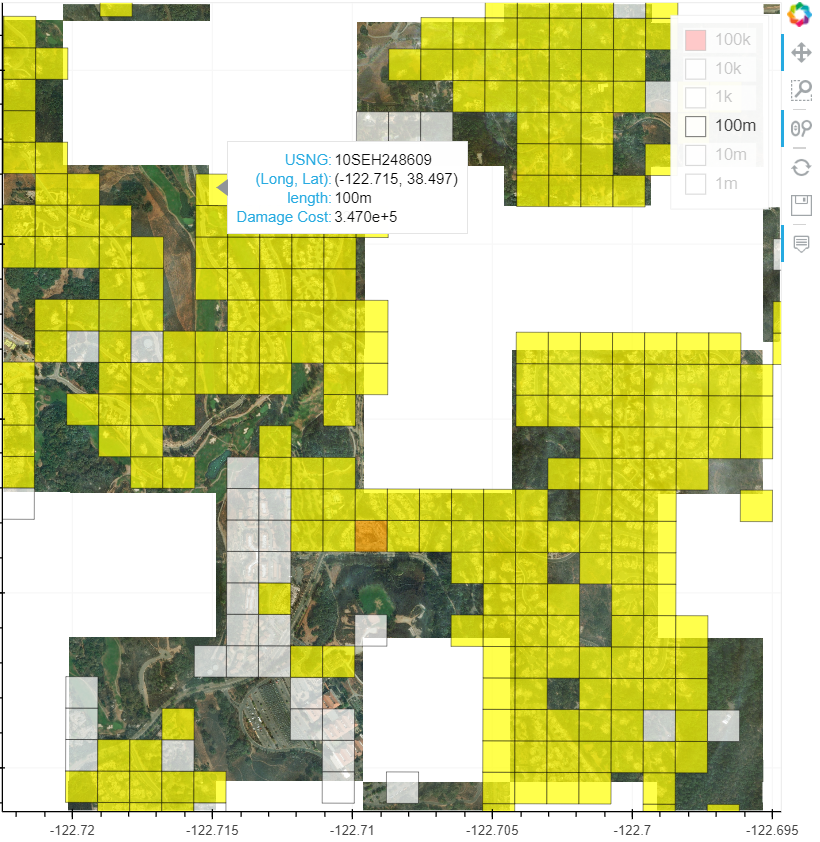
\includegraphics[width=1\linewidth]{Bokeh.png}
\caption{Bokeh xBD USNG Visualization}
\label{bokehplot}
\end{figure}




\section{Final Application}
\subsection{Overview}
The resulting efforts from the damage classification algorithms and financial modeling were integrated into a proof-of-concept application. Due to time constraints, a minimum viable product damage classification model was trained using a modified U-Net architecture developed by the AI for Humanitarian Assistance and Disaster Relief \cite{a17}. This damage model outputs a pixel level damage estimation according to the xBD classifications. The application functions by having a user upload an image of an area before and after a disaster, along with the latitude and longitude coordinates of the image, then the damage classifier assess the damage level of each pixel and financial costs of the damage are visualized according to the USNG at all levels of precision. This application will enable images of disaster areas to be quickly assessed and relevant financial feedback provided to inform disaster relief\footnote{ This visualization is hosted at test-env.eba-6qua3x4j.us-east-1.elasticbeanstalk.com and made available upon request}.

\begin{figure}[htbp]
\centering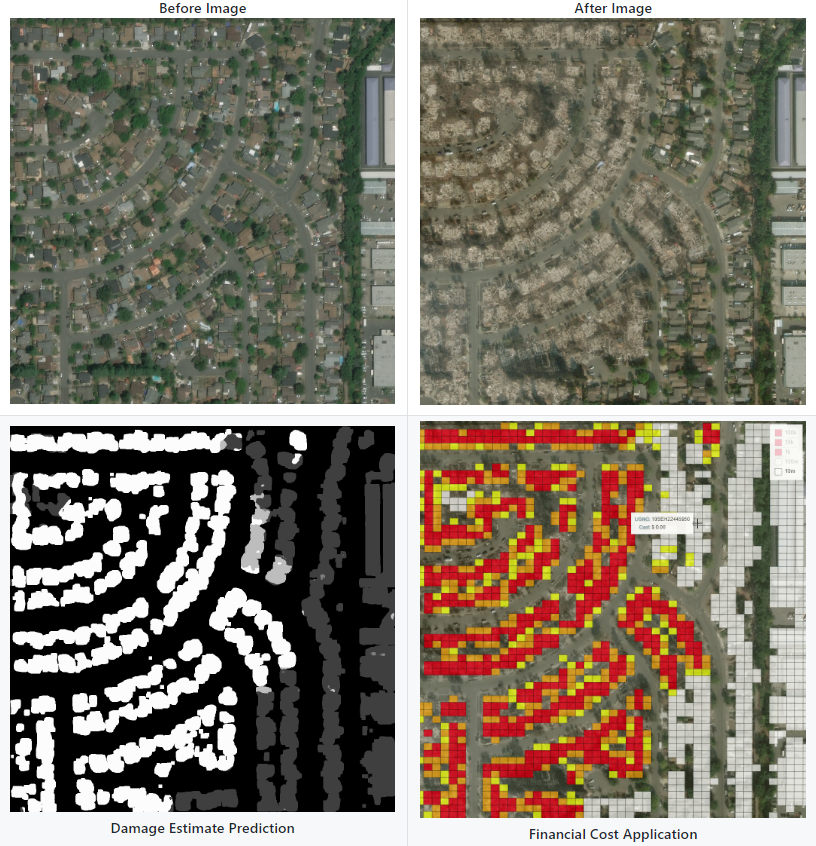
\includegraphics[width=1\linewidth]{applicationcombined.png}
\caption{Application Workflow}
\label{appworkflow}
\end{figure}

\subsection{Methods}
Application processing beings by first taking the uploaded images of a damaged location and running the damage classification model to return a pixel level damage estimate. Fig.~\ref{appworkflow} includes the inputted before/after images, the outputted damage estimate pixel predictions and the final application. Next, these pixel images are binarized and polygons for each building are determined using OpenCV. 

Originally, the financial model would have processed as described above --- finding the centroids and areas of each polygon, finding respective USNG grids and then sum financial costs over all grids --- however an issue arose with this approach. The damage model tended to connect buildings which were nearby into a single, large building. This resulted in centroids which represented groups of buildings and an inaccurate listing of the USNG grids present in the image. To combat this, the obtained polygons are further subdivided into smaller polygons along their largest dimensions until the width of any polygon is less than a certain number of pixels. This ensures that by taking the centroids of each polygon all of the ten meter USNG precision levels within the image are captured. An image of the subdivided polygons is shown in Fig.~\ref{subdivide}.



Once building polygons are established, the \emph{mgrs} module is applied to the centroid of each and the lat/lons polygons of each USNG grid are obtained using the plotting function for all precision levels as described earlier. The latitude and longitude values of the USNG polygons are then into image pixel coordinates. This is done using the resolution of the uploaded images and the inputted image lat/lon values to determine a change in latitude/longitude per pixel and then scaling and translating each point in the USNG polygons. Linear interpolation is done to connect the USNG polygon corners within the image coordinates. 

\begin{figure}[ht]
\centering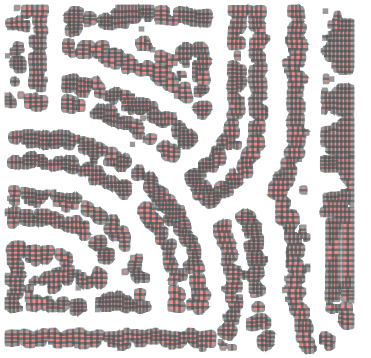
\includegraphics[width=0.7\linewidth]{subdividedpolygons.png}
\caption{Subdivided Polygons}
\label{subdivide}
\end{figure}

With USNG polygons obtained in image coordinates, the financial model described above is applied on a pixel by pixel level to obtain the final cost estimates. An area per pixel is calculated by diving the total image area by the resolution. The cost per square foot is obtained using the Zillow data and the zipcode of the image. Image pixel values are converted from damage classes (i.e., 0-3) to damage level factors within the financial model (i.e., 0, 0.5, 0.8, and 1). A image of this process is shown visually in Fig.~\ref{pixelmodel} This multiplication is performed on all pixels within each USNG grid to obtain estimated cost values utilized in the final visualization.

\begin{figure}[h]
\centering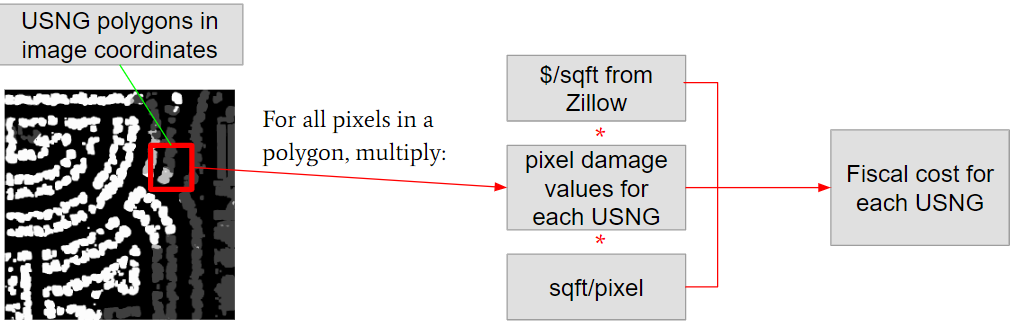
\includegraphics[width=1\linewidth]{appmultiply.png}
\caption{Pixel Based Financial Model}
\label{pixelmodel}
\end{figure}

\subsection{Performance}
Computation speed and estimation accuracy were a principal concerns in the application design. The application was hosted on Amazon Web Services (AWS) on a single core, dual threaded t3a.small instance. Damage classification was performed with frozen weights in around 5 seconds. The financial modeling and rendering process was performed in approximately 20 seconds. Implementation on four core machines have seen total processing times around 10 seconds with the use of multiprocessing. The estimations appear to be roughly representative of damage estimates at the 10 meter level of precision and above. While computing at the one meter level of precision is theoretically possible, issues with ground sampling distance of the images being greater than a single meter render the results inaccurate and an unreasonable computational time is required.

\section{Conclusions}
This paper sets out the design and implementation of a proof-of-concept natural disaster geospatial damage assessment application. Various modeling techniques were explored to automatically classify building damage from satellite images. A pixel based financial model and a mapping function for the United States National grid created. These aspects were integrated together into an application which allows fast identification and visualization of damage costs associated with a region to expedite and inform relief efforts.

\section*{Acknowledgment}

This work is the result of a collaborative partnership between George Mason University and Accenture Federal Services. Particular acknowledgements are given to Rajesh Aggarwal, Marc Bosch Ruiz, Christian Conroy, James Baldo, and Brett Berlin.  

\begin{thebibliography}{00}
\bibitem{a1} R. Gupta, R. Hosfelt, S. Sajeev, N. Patel, B. Goodman, J. Doshi, E. Heim, H. Choset and M. Gaston. xBD: A dataset for assessing building damage from satellite imagery. \emph{arXiv:1911.09296 [cs.CV]}, Nov. 2019.
\bibitem{a3}A. Fujita, K. Sakurada, T. Imaizumi, R. Ito, S. Hikosaka and R. Nakamura. Damage detection from aerial images via convolutional neural networks. \emph{2017 Fifteenth IAPR International Conference on Machine Vision Applications (MVA)}, pages 5--8, Nagoya, Japan, May 2017. IEEE.
\bibitem{a4} J. Xu, W. Lu, Z. Li, P. Khaitan and V. Zaytseva. Building damage detection in satellite imagery using convolutional neural networks. \emph{arXiv:1910.06444 [cs.CV]}, Oct. 2019.
\bibitem{a5} J. Doshi, S. Basu and G. Pang. From satellite imagery to disaster insights. \emph{arXiv:1812.07033 [cs.CV]}, Dec. 2018.
\bibitem{a6} A. Krizhevsky, I. Sutskever and G. E. Hinton. Imagenet classification with deep convolutional neural networks. \emph{Commun. ACM}, 60(6):84–90, May 2017.
\bibitem{a7} M. Ji, L. Liu and M. Buchroithner. Identifying collapsed buildings using post-earthquake satellite imagery and convolutional neural networks: A case study of the 2010 Haiti earthquake. \emph{Remote Sens.}, 10(11):1689, Oct. 2018.
\bibitem{a8} F. N. Iandola, S. Han, M. W. Moskewicz, K. Ashraf, W. J. Dally and K. Keutzer. SqueezeNet: AlexNet-level accuracy with 50x fewer parameters and \textless0.5MB model size. \emph{arXiv:1602.07360 [cs.CV]}, Feb. 2016.
\bibitem{a2} O. Ronneberger, P. Fisher and T. Brox. U-Net: Convolutional networks for biomedical image segmentation.\emph{arXiv:1505.04597 [cs.CV]}, May 2015.
\bibitem{a18} Kaiming He,Georgia Gkioxari, Piotr Dollar, Ross Girshick. Mask R-CNN: Facebook AI Research (FAIR) \emph{arXiv:1703.06870 [cs.CV]}, Jan. 2018.
\bibitem{a19} Waleed Abdulla.Mask R-CNN for object detection and instance segmentation on Keras and TensorFlow "https://github.com/matterport/MaskRCNN"
\bibitem{a9} C. H. Sudre, W. Li, T. Vercauteren, S. Ourselin, and M. J. Cardoso, “Generalised dice overlap as a deep learning loss function for highly
unbalanced segmentations,” arXiv:1707.03237, 2017.
\bibitem{a10} Clinton County Ohio, “United States National Grid”, http://www.clintoncountyohgis.org/Maps/MapsIndex/Pages/MapsU/...
united\_states\_national\_grid.html, 2020.
\bibitem{a11} Federal Geographic Data Committee, “United States National Grid”, https://www.fgdc.gov/usng, 2020.
\bibitem{a12} Howard Butlet, “mgrs” https://pypi.org/project/mgrs/, 2011.
\bibitem{a13} National Geospatial-Inteligence Agency, “MSP Geotrans Assistance” https://earth-info.nga.mil/GandG/update/index.php?action=home, 2020.
\bibitem{a14} Zillow Research, “Zillow Home Value Index” https://www.zillow.com/research/data/, 2018.
\bibitem{a15} United States Census Bureau, “Geography Program” https://www.census.gov/programs-surveys/geography.html, 2020.
\bibitem{a16} National Ocean and Atomosphereic Administration, “Billion-Dollar Weather and Climate Disasters: Events”, https://www.ncdc.noaa.gov/billions/events, 2020.
\bibitem{a17} AI for Humanitarian Assistance and Disaster Relief, “xView2unet”, https://github.com/canktech/xview2unet, 2020.

%make sure bib items are in order
\end{thebibliography}
\vspace{12pt}
\newpage
\pagebreak
\newpage
\section*{Appendix}
Other content related to class requirements are placed here. Image for xBD class imbalance is found in Fig.~\ref{xviewimbal}. A Leaflet plot of a particular county within xBD where the data is not representative of the entire county damage is found in Fig.~\ref{xviewleaflet}. An additional visualization of the xView2 data is found at https://tyler-richardett.github.io/gmu_daen_690_capstone/. 

\subsection{Xview2 Dataset Analysis}
\textbullet Description:
The provided dataset includes various parameters. For a complete listing of the parameters available in the Xview2 dataset view Fig.~\ref{xviewattr}. 

\subsubsection{Data Conditioning}
Much of the data conditioning tasks have been performed by the dataset providers. The baseline solution provides much of the preprocessing steps needed in the classification pipeline (e.g., mask generation, building polygon separation, etc.). Additionally, other confounding factors, such as high cloud coverage have been eliminated in the dataset.

\subsubsection{Data Quality Assessment} \\
\textbullet Completeness: The dataset includes 19 different disasters, but does not include every building destroyed in each disaster, only a sampling.\\
\textbullet Uniqueness: Six different disaster types are available, with a variety of the number of buildings in each image. Some images have tens of buildings and others have none at all.\\
\textbullet Accuracy: Annotations passed through many phases of review by many annotations and randomly sampled and evaluated by experts from California Air National Guard, NASA, and FEMA. \\
\textbullet Atomicity: The damage classification evaluations are available on a building by building level with only 4 discrete levels of damage.\\
\textbullet Conformity:Properly ordered as set by the competition data providers in a consistent format.\\
\textbullet Overall Quality: Excellent. Predictions will be difficult by off-nadir axis images and difficulty to tell the difference between major and minor damage using satellite images, but this is intended by the competition and is not an issue with the data itself.

\subsubsection{Risks} \\
\textbullet Some of the potential risks which were associated with the project: inability to find valuable datasets containing disaster cost information, difficulty applying these costs without having a subject matter expert in this domain, and being unable to develop an algorithm to detect objects other than buildings and the resulting damage caused and conflating this information with property damage costs for validation. The financial analysis model is based on several assumptions which will help simplify the model as economic loss data has heavy variance with respect to the region and type of disaster. Also, other object damage loss is not included in our dataset. Considerations such as transportation, obstructions, and demolition costs, raw material price fluctuations, and the like are all factors that will need to be accurately modeled based on the poor validation data we obtained based on our underlying assumptions. 


\begin{figure}[h]
\centering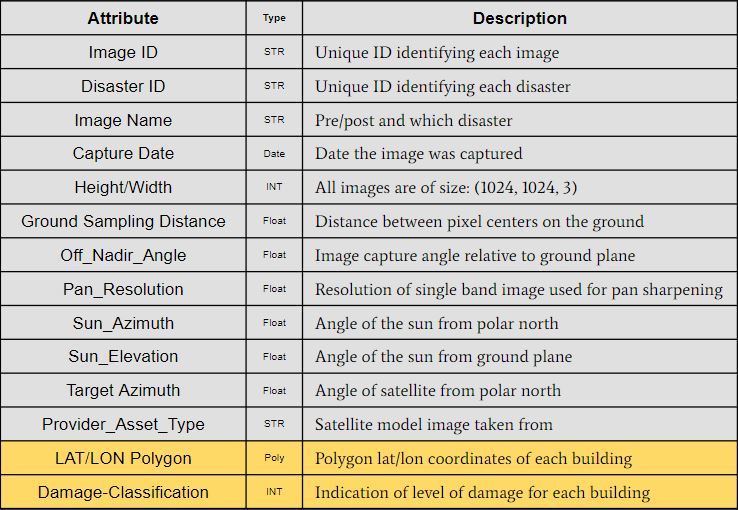
\includegraphics[width=1\linewidth]{data.JPG}
\caption{xView2 Data Attributes}
\label{xviewattr}
\end{figure}

\begin{figure}[ht]
\centering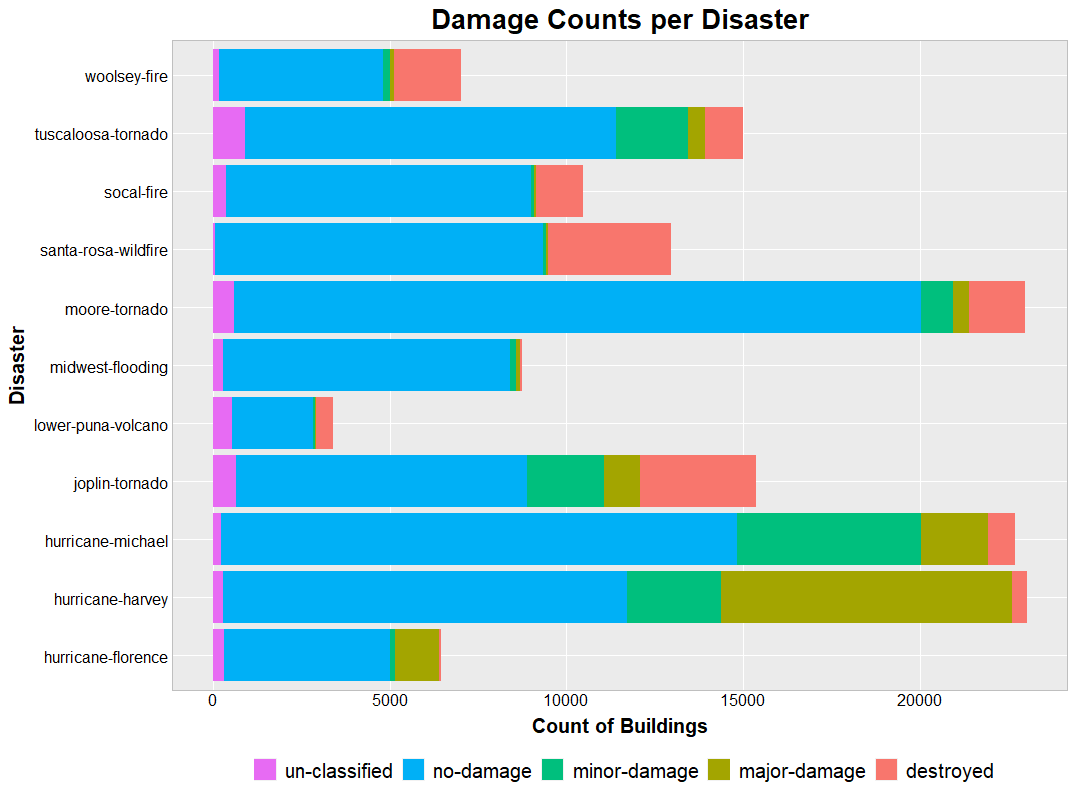
\includegraphics[width=1\linewidth]{imbalanced.png}
\caption{xView2 Class Imbalance}
\label{xviewimbal}
\end{figure}

\begin{figure}[ht]
\centering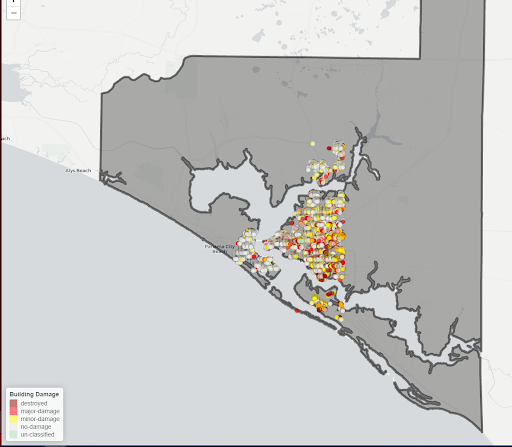
\includegraphics[width=1\linewidth]{leaflet.png}
\caption{xView2 Disaster v. County}
\label{xviewleaflet}
\end{figure}

\end{document}
